\chapter{Materiais e Métodos}

\section{Modelo da rede neural DG-CA3}




\begin{figure}
    \centering
    \caption{Arquitetura da rede}
    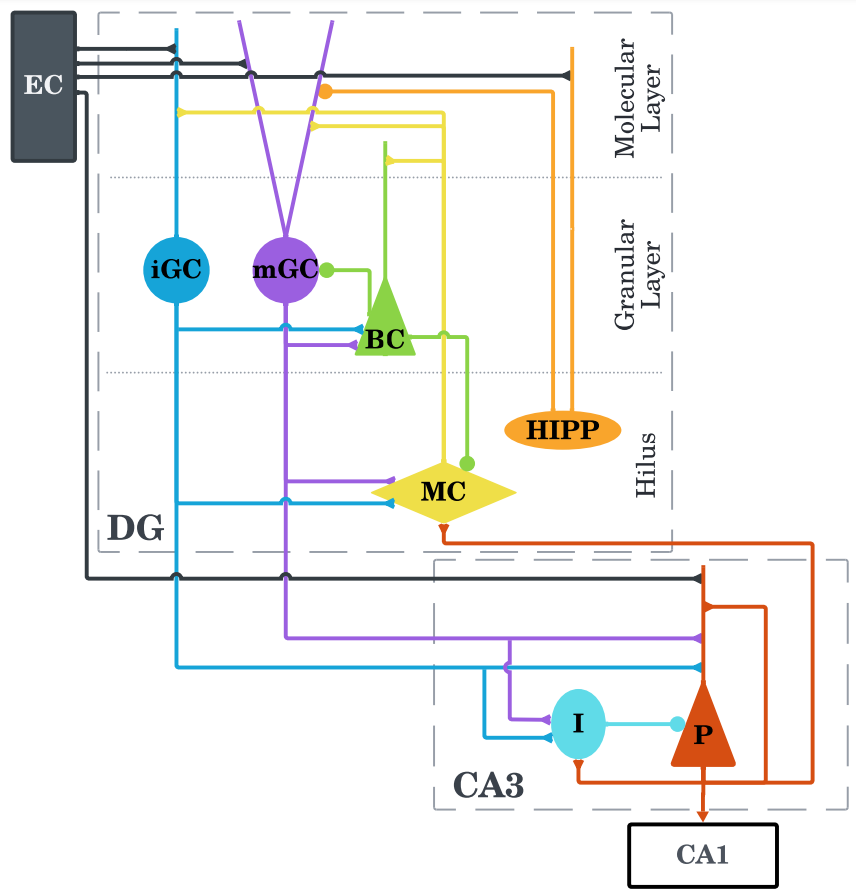
\includegraphics[scale=0.7]{figuras/arquitetura-rede.png}
    \label{fig:arquitetura-rede}
\end{figure}


\section{Modelo de neurônio}

Os neurônios foram modelados de acordo com o modelo de neurônio de Izhikevich de 9 parâmetros~\cite[cap.~8]{izhikevichDynamical2006}.






